\revision{To achieve the desiderata in \cref{sec:cant_have_it_all}, we propose a new rate measure. We first detail our new rate measure. Then we provide intuition for its choice and describe the role of its (hyper)parameters. Finally we show that the resulting two-population model (\cref{eq:generative_model}) satisfies \cref{req:finite_mean,req:inf_mass}.}

In what follows, we propose to use the two-population model with the following PPP rate measure on the variant frequencies:
\begin{equation}
	\ratemeasproposed(\de\vecvariantfreq{}) := \mass
			\frac{(\variantfreqperpop{1}+\variantfreqperpop{2}^{\rate{2}/\rate{1}})^{-\rate{1}}}{(\variantfreqperpop{1}+\variantfreqperpop{2})^{\corr{1}+\corr{2}}}
			\frac{\variantfreqperpop{1}^{\corr{1}-1}(1-\variantfreqperpop{1})^{\conc{1}-1}}{B(\corr{1}, \conc{1})}\frac{\variantfreqperpop{2}^{\corr{2}-1}(1-\variantfreqperpop{2})^{\conc{2}-1}}{B(\corr{2}, \conc{2})} \bm{1}_{[0,1]^2} (\vecvariantfreq{}) \de\btheta.
	\label{eq:proposed_prior}
\end{equation}
Here $B(\cdot, \cdot)$ denotes the beta function. 
The measure $\levync$ is characterized by seven scalar hyperparameters, which we collect in the vector $\allhyper := (\mass, \rate{1}, \rate{2}, \corr{1}, \corr{2}, \conc{1}, \conc{2})$.

Before discussing the \revision{hyperparameter roles below}, we observe that our rate measure takes the form of the product rate measure $\levytbp(\de\variantfreqperpop{1}) \levytbp(\de\variantfreqperpop{2})$ multiplied by a term that does not factorize into components unique to 
frequencies in population 1 and 2. 
A rough intuition for our choice of $\ratemeasproposed$ is that first, we wish to retain a product of beta distributions to ensure conjugacy.
Second, we observe that, per \cref{prop:incomp}, we need a leading factor before the beta-distribution product that does not factorize. Moreover,
we need to choose the leading factor in a way that satisfies \cref{req:finite_mean,req:inf_mass} and also allows desirable power law growth properties (\cref{sec:powerlaw}). We describe how we arrived at the particular choice of $\ratemeasproposed$ in more detail in \cref{sec:prior_construction_details}.

\revision{Next, we describe the roles of the various hyperparameters in $\ratemeasproposed.$}
The \emph{mass} parameter $\mass>0$ has the same role as in the (one-population) 3BP rate measure. \revision{Namely, it linearly scales
the expected number of total variants for finite $\vecsamplesize$; for a precise statement, see \cref{eqn:kr_tons} in \cref{prop:predict_kr_tons}}.

In the one-population case, the number of unique variants grows according to a power law as a function of the number of samples \citep{Broderick2012, Masoero2022}, and the single \emph{rate} parameter $\rate{}$ controls the power-law rate. In the two-population model with our new rate measure, growth of the number of variants has a more complex dependence on the number of samples since $\vecsamplesize$ can vary by different amounts in each population. But the rate parameters $\rate{1}, \rate{2} \in (0,1)$ can again be seen to control a notion of power-law growth in each population; we elaborate on the details in \cref{sec:powerlaw}.

Analogous to the one-population case, the \emph{concentration} parameters $\conc{1}, \conc{2} > 0$ modulate the frequencies of common variants; in particular, as $\conc{\popidx}$ grows large, population $\popidx$ is less likely to have variants whose frequencies are close to 1.

The \emph{correlation} parameters $\corr{1}, \corr{2} > 0$ do not have an analogue in the single-population case since they control the
\revision{correlation between each variant's frequency in one population and its frequency in the other. We illustrate some potential correlation
structures in \Cref{fig:log_rate_sigma}. When both $\corr{1}, \corr{2}$ are small (\Cref{fig:log_rate_sigma}, left), variant frequencies are negatively correlated
across populations; when variants have a high frequency in one population, they tend to have a low frequency in the other population. 
When both $\corr{1}, \corr{2}$ are large (\Cref{fig:log_rate_sigma}, right), variant frequencies are positively correlated
across populations. When $\corr{1}, \corr{2}$ differ substantially (\Cref{fig:log_rate_sigma}, center), variants tend to be more frequent
in the population with the larger $\corr{}$ value.}


\begin{figure}
    \centering
    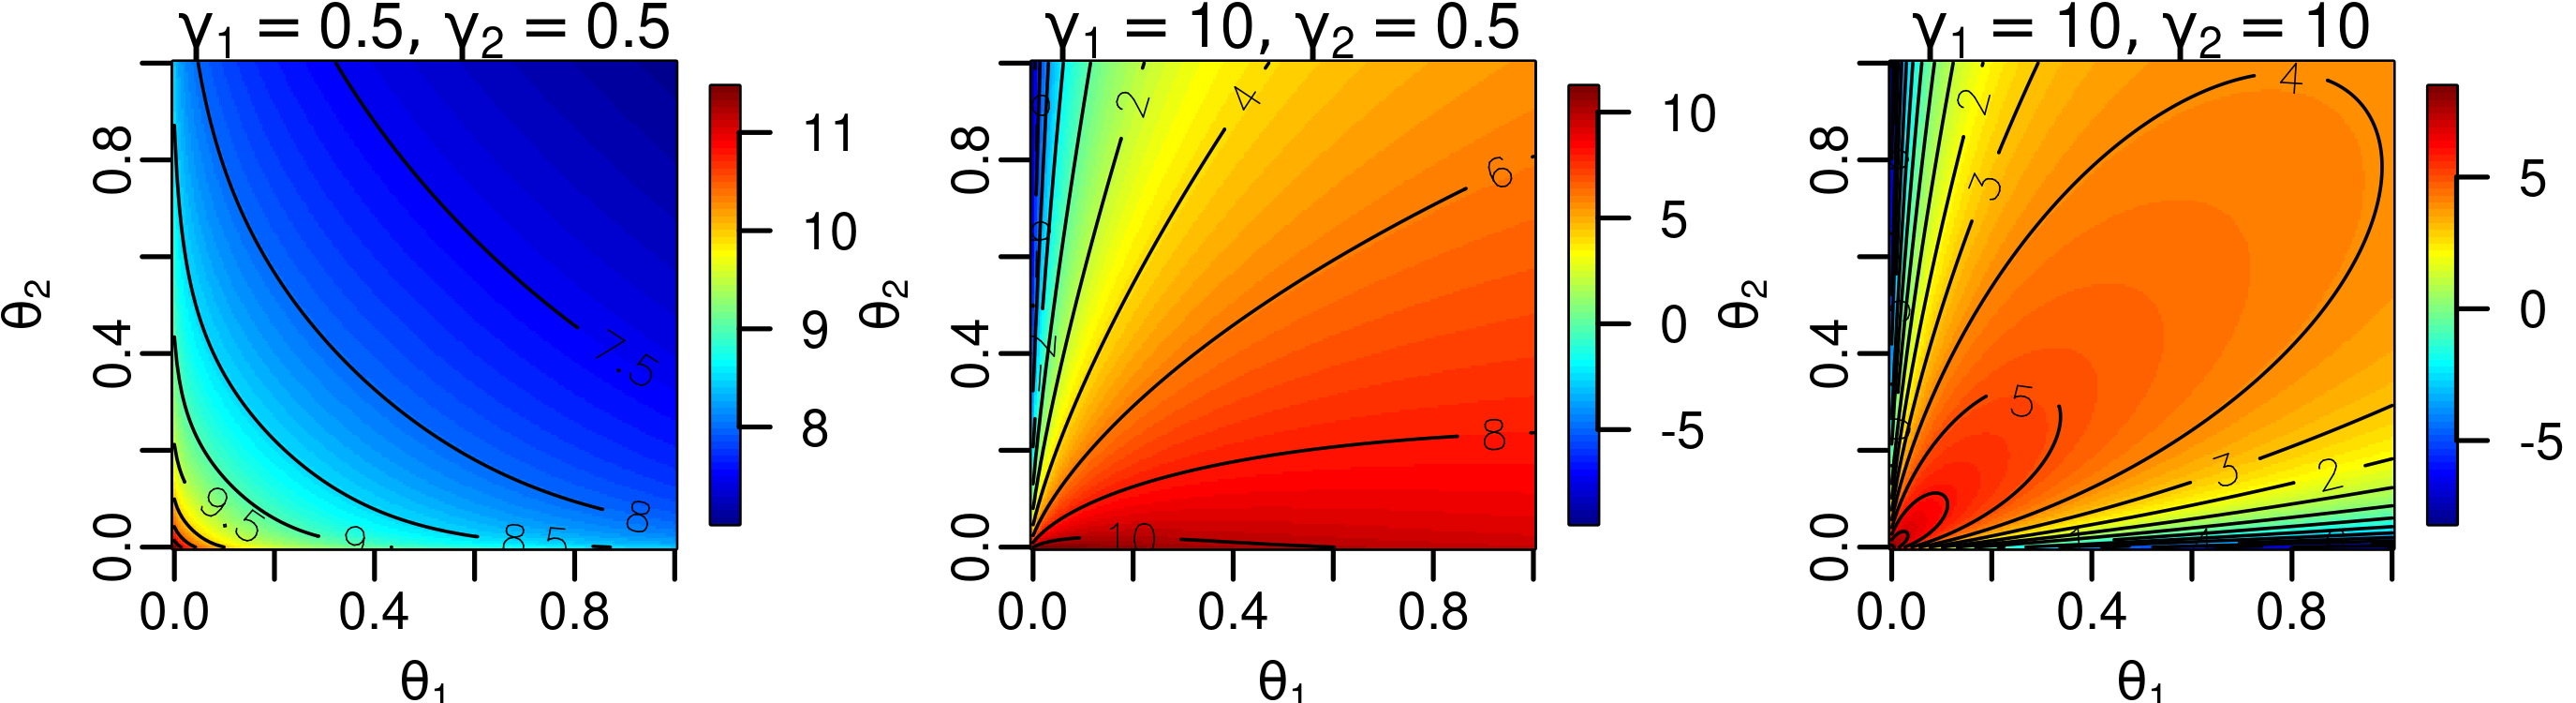
\includegraphics[width = \linewidth]{Ch2-double-trouble/Figs/rate_measures_near_cojugate.png}
    \caption{Visualization of the log density of our proposed rate measure in \cref{eq:proposed_prior} with different values of the $\corr{1},\corr{2}$ hyperparameters. In all plots, the other hyperparameters are $\rate{1}=\rate{2}=0.2, \conc{1}=\conc{2}=1$, and $\mass = 1$.}
	\label{fig:log_rate_sigma}
\end{figure}


Our next result verifies that the hyperparameter ranges here are sufficient to ensure our desiderata;
see \cref{sec:proper_proof} for a proof. \minorrevision{An interesting line of investigation for future work would be to establish hyperparameter ranges that are both sufficient and necessary.}
\begin{myProposition} \label{prop:hyperparams}
If the hyperparameters satisfy $\mass, \conc{1}, \conc{2}, \corr{1}, \corr{2}>0$ and $\rate{1}, \rate{2} \in (0,1)$, the two-population model (\cref{eq:generative_model}) satisfies \cref{req:finite_mean,req:inf_mass} when paired with our rate measure $\ratemeasproposed$ from \cref{eq:proposed_prior}.
\end{myProposition}

A common challenge in BNP is computation with the countably infinite set of parameters implied by \cref{req:inf_mass}.
Like typical models used in practice, though, our model enjoys conjugacy. Namely, analogous to the one-population model from \citet{Masoero2022}, our rate measure in \cref{eq:proposed_prior} is an exponential family conjugate prior for the Bernoulli process likelihood in the sense of \citet{Broderick2018}. We thereby avoid any infinite-dimensional integrals. See Section \cref{app:conjugacy} for a formal account and proof. 

